% Overview : intro.tex
% Explain why this talk is being given.

\begin{frame}[ctb!]
  \frametitle{Introduction : Purpose}
  Fuel cycle simulators are designed to answer policy-related questions
  regarding transitions from one equilibrium state to another.

  \vspace{0.2cm}

  \pause
  A simulator answers the following questions as a function of its 
  parameter space:
  \begin{itemize}
    \item how much material exists
    \item where does that material reside
    \item from/to where and when is material transported
    \item what kinds of facilities are needed
    \item when is each type of facility needed
  \end{itemize}
\end{frame}

\begin{frame}[ctb!]
  \frametitle{Introduction : VISION}
  VISION is one such simulator developed at INL and used by the DOE. 
  It is well represented in the literature and can model most aspects 
  of the fuel cycle. \cite{yacout_vision_2006}
  \begin{itemize}
    \item continuous material flows
    \item fleet-based facility deployment
    \item some regional modeling capability
    \item input/output via Excel
    \item simulation engine via Powersim
  \end{itemize}
\end{frame}

\begin{frame}[ctb!]
  \frametitle{Introduction : Cyclus}
  Cyclus is a fuel cycle simulator implemented as an agent-based model,
  i.e., entities are defined separately and then interact. Output 
  metrics are simply an aggregation of those interactions.

  \vspace{0.4cm}

  This approach has been chosen because it allows for encapsulation of
  agent behavior. The simulation engine in conjunction with this 
  encapsulation provides a common fuel cycle simulator framework, i.e.
  a common simulator language.

  \vspace{0.4cm}

  \pause
  This discussion will showcase capability additions to the Cyclus
  simulation engine and the modules that use them. We then provide a
  use case example of both Cyclus and Vision via the INPRO 
  Business-as-Usual (BAU) once-through benchmark.
\end{frame}

\begin{frame}[ctb!]
  \frametitle{Introduction : Benchmark}
  The INPRO BAU benchmark specifies that two types of reactors will
  be built based upon demand for energy.
  \begin{figure}[htbp!]
    \begin{center}
      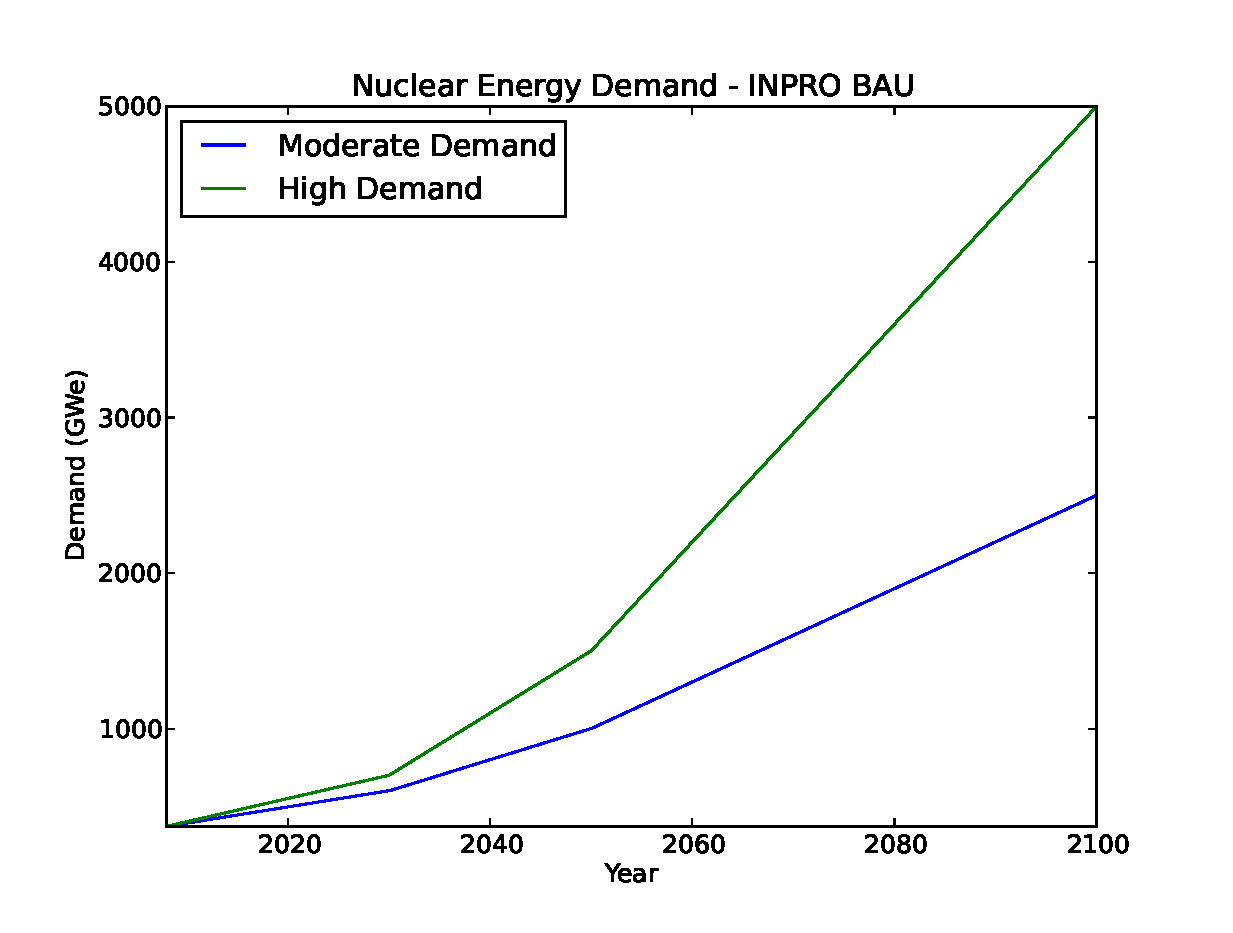
\includegraphics[height=4cm]{inpro-demand.eps}
    \caption{The energy demand specification for the INRPO BAU scenarios.}
    \label{fig:inpro-demand}
    \end{center}  
  \end{figure}
  Reactor deployment is split between LWRs (94\% of energy demand) and
  HWRs (6\% of energy demand). Reactors have a 40 year operation lifetime.
\end{frame}
